\chapter{Analysis} \label{chap:Analysis}

%TODO: edit this awkwardness
The ORCAS tool is analyzed by looking at three case studies. 
We created three instrument types: Spectrometer, High Resolution Spectrometer, and FX Correlator, as defined in Sections \ref{Real Time Radio Astronomy Algorithms:Spectroscopy}, \ref{Real Time Radio Astronomy Algorithms:Pulsar Processing}, and \ref{Real Time Radio Astronomy Algorithms:Correlation}. 
Each case study was chosen to illustrate a different aspect of the toolflow.
The spectrometer gives an example of the end to end toolflow using a simple dataflow, the high resolution spectrometer allows us to explore tradeoffs in the design space and the FX correlator shows how the tool behaves when designing very large instruments.


%Simple spectrometer placement

%TODO: Include appropriate FFT or PFB benchmarks

%Summary: describe how we get real numbers to put into previous part
%Goal: define and obtain real numbers from the previous part
%\section{Benchmarks}

%\subsection{Cost}

%Summary: case studies describing partitioning of realistic-scale instruments
%Goal: show successful application of tool to design of realistic instruments
%provide analysis comparing this to hand-designed instruments 
\section{Spectrometer Case Study}
The spectrometer is a simple instrument, making it easy to follow the end to end toolflow.
We design %a 50 MHz and 
an 800 MHz spectrometer that breaks the band into 1024 channels.
%TODO: what is a reasonable integration time here


\subsection{Spectrometer Definition}
Defining a simple spectrometer requires very few parameters. 
First, as with most instruments, the astronomer must specify the sky bandwidth the instrument must process, defined in MHz and the number of bits in each ADC sample.
Then, the desired spectral resolution is defined in MHz per channel, or analogously, the number of channels that should be used to break up the bandwidth.
Finally, the integration time needs to be defined.

One optional parameter, number of antennas, can also be defined. 
This describes the number of independent spectrometers that need to be created.
While this parameter does not affect the end to end processing for each antenna, knowing how many spectrometers are needed allows for more efficient use of the hardware.

The 800 MHz spectrometer is created simply by defining the parameters and instantiating a Spectrometer object as follows:

\lstinputlisting[language=Python,
    %caption=My Class,
    label={spec_defn.py},
    breaklines=true,
  ]{code/C6/spec_defn.py}

\subsection{Spectrometer Dataflow}

%TODO: add detection step
\begin{figure}[ht!]
  \centering
    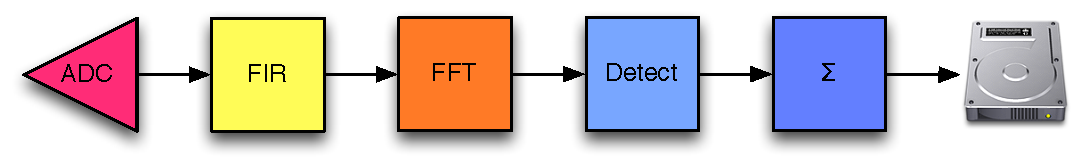
\includegraphics[width=1\textwidth]{Images/C4/spectrometer_dataflow.pdf}
  \caption{General Spectrometer Dataflow Model}
  \label{fig: C4/spectrometer_dataflow.pdf}
\end{figure}

The spectrometer instrument definition generates a very simple dataflow. 
Figure \ref{fig: C4/spectrometer_dataflow.pdf} shows the general dataflow model for a single antenna spectrometer. 
This model can be applied to any spectrometer, as the spectrometer parameters do not affect how many computational blocks are required or the interconnect layout. 
The ADC feeds data into a FIR filter. 
Then the filtered signal is transformed into channels in the FFT and those channels are accumulated and saved to disk. Regardless of the parameters the astronomer chooses, the dataflow will be the same. 

The parameters for each block come directly from the instrument definition. 
The FIR parameters come from the number of FIR taps and window shape, the FFT is simply defined by the FFT length parameter and the accumulator also is parameterized by the FFT length as well as the integration time. 
The code below shows how the blocks are added to the dataflow model.

\lstinputlisting[language=Python,
    %caption=My Class,
    label={spec_dflow.py},
    breaklines=true,
  ]{code/C6/spec_dflow.py}

\subsection{Spectrometer Mapping}
As a simple case study, an 1024 channel 800 MHz spectrometer is mapped using the ROACH and GTX 580-based NRAO server as potential platforms. 
ORCAS produces a solution that maps the entire design to a single ROACH board.
This solution is obviously correct since the bandwidth cannot be processed by a single GPU and a single ROACH is cheaper than a combination of boards.
The mapping produced by ORCAS is shown below.

\lstinputlisting[
    %caption=My Class,
    label={spec_dflow.py},
    breaklines=true,
  ]{code/C6/spec_800_result.txt}
  

%\lstinputlisting[
%    %caption=My Class,
%    label={spec_dflow.py},
%    breaklines=true,
%  ]{code/C6/spec_050_result.txt}
  
%\subsection{Cost}
%\subsection{Power}

\section{High Resolution Spectrometer Case Study}
The high resolution spectrometer is a useful instrument for SETI. 
The two stage channelization creates a large number of channels without using an FFT that is too large to fit on a single board.


\subsection{High Resolution Spectrometer Definition}
The main difference between a spectrometer and a high resolution spectrometer is the need for two stages of channelization rather than just one. 
The sky bandwidth, integration time, and number of antennas are defined in the same way as the previous spectrometer type. 

The spectral resolution is defined differently, because both the coarse and fine resolutions need to be defined. 
The coarse resolution defines how many channels the whole sky bandwidth should be broken up into initially.
The fine resolution defines how many channels each coarse channel is broken into.
Both can be described in MHz per channel.

\subsection{High Resolution Spectrometer Dataflow}

%TODO: add detection step
\begin{figure}[ht!]
  \centering
    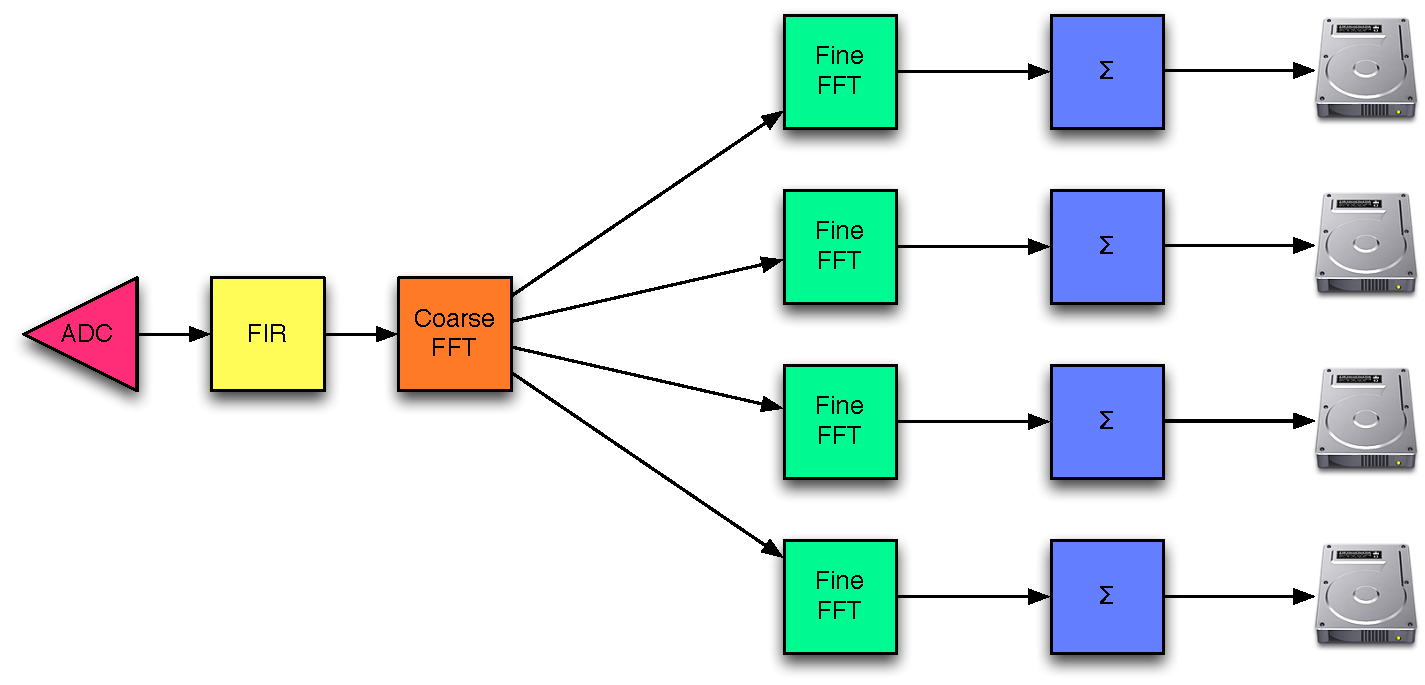
\includegraphics[width=1\textwidth]{Images/C4/hires_spectrometer_dataflow.pdf}
  \caption[Example High Resolution Spectrometer Dataflow Model]{Example High Resolution Spectrometer Dataflow Model
  \textit{
  This figure shows an example dataflow for a high resolution spectrometer with 4 coarse FFT channels.
  Like the previous spectrometer, the data comes in through an ADC, is filtered and then channelized using a coarse FFT.
  Then, to achieve a higher resolution, each coarse channel is divided into sub-channels using the 4 fine FFT blocks in the dataflow. 
  }}

  \label{fig: C4/hires_spectrometer_dataflow.pdf}
\end{figure}

The high resolution spectrometer dataflow does depend on the parameters specified in the instrument description. 
An example dataflow is shown in Figure \ref{fig: C4/hires_spectrometer_dataflow.pdf}. 
The first three blocks in the dataflow are exactly the same as the Spectrometer dataflow described in the previous section. 
An ADC feeds data into a FIR filter followed by an FFT. 
After the FFT, the algorithm is modified to accommodate the higher resolution required. 
The first FFT divides the band into a number of coarse channels and then each coarse channel must be further divided into a number of fine channels. 
The coarse FFT must feed its data to a separate fine FFT for each coarse channel, so the number of fine FFTs in the dataflow diagram will vary based on the number of coarse channels.
At this point, each coarse channel is processed in an independent pipeline the finely channelized data is accumulated and recorded to disk. 
The example in Figure \ref{fig: C4/hires_spectrometer_dataflow.pdf} shows a spectrometer that divides the data into 4 coarse channels.

%\subsection{Cost}
%\subsection{Power}

\subsection{Algorithmic Exploration}

The Arecibo L-band feed array, pictured in Figure \ref{fig: C3/alfa_feed.png} has 7 dual-polarization beams. 
The SERENDIP V.v instrument was only able to process one beam at a time, but its planned successor, SERENDIP 6, will process 300MHz from each beam-pol.

\begin{figure}[ht!]
  \centering
    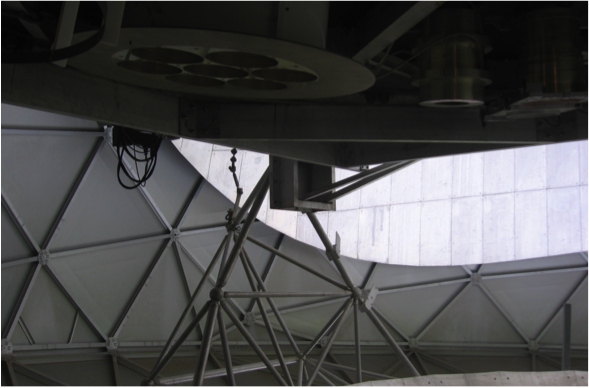
\includegraphics[width=\textwidth]{Images/C3/alfa_feed.png}
  \caption{Arecibo ALFA Feed}
  \label{fig: C3/alfa_feed.png}
\end{figure}

In this case study, we analyze the design space for a 300 MHz 256 million channel spectrometer, similar to the SERENDIP 6 instrument.
This instrument provides an interesting case study because the number of channels is so large.
The number of channels in the coarse and fine FFTs can be varied, as long as the product remains 256 million.
We explore this design space by varying the dimensions and number of antennas to see how the channel balance affects the final cost of the instrument.

This instrument is designed using ROACH boards and the GTX 580-based NRAO server as supported platforms, and uses the FIR and FFT benchmarks presented in Chapter \ref{chap:Algorithm Partitioning}
To aid the linear program, we assume reordering the coarse FFT data is infeasible on the GPU and force the design to reorder the data on the FPGA.


\begin{sidewaystable}
\begin{tabular}{| c | c | c | c | c | c |}
\hline  
\diaghead{\theadfont Diag ColumnmnHead II}{\textbf{Antennas}}{\textbf{Dimensions}} & 256 by 524,288 & 512 by 262,144 & 1024 by 131,072 & 
2048 by 65,536 & 4096 by 32,768\\
\hline  
1 &  \begin{tabular}{c} 2 GPUs \\ 1 ROACH \\ \$13.7k \end{tabular} & \begin{tabular}{c} 2 GPUs \\ 1 ROACH \\ \$13.7k \end{tabular} & \begin{tabular}{c} 2 GPUs \\ 1 ROACH \\ \$13.7k \end{tabular} & \begin{tabular}{c} 1 GPU \\ 1 ROACH \\ \$10.2k \end{tabular} &\begin{tabular}{c} 1 GPU \\ 1 ROACH \\ \$10.2k \end{tabular}  \\
\hline
3  & \begin{tabular}{c} 5 GPUs \\ 1 ROACH \\ \$24.2k \end{tabular} & \begin{tabular}{c} 4 GPUs \\ 1 ROACH \\ \$20.7k \end{tabular} & \begin{tabular}{c} 4 GPUs \\ 1 ROACH \\ \$20.7k \end{tabular} & \begin{tabular}{c} 3 GPUs \\ 1 ROACH \\ \$17.2k \end{tabular} & \begin{tabular}{c} 3 GPUs \\ 2 ROACH \\ \$23.9k \end{tabular} \\
\hline  
5 & \begin{tabular}{c} 8 GPUs \\ 2 ROACH \\ \$41.4k \end{tabular} & \begin{tabular}{c} 7 GPUs \\ 2 ROACH \\ \$37.9k \end{tabular} & \begin{tabular}{c} 7 GPUs \\ 2 ROACH \\ \$37.9k \end{tabular} &
 \begin{tabular}{c} 5 GPUs \\ 2 ROACH \\ \$30.9k \end{tabular} &  \begin{tabular}{c} 5 GPUs \\ 2 ROACH \\ \$30.9k \end{tabular} \\
\hline  
7 & \begin{tabular}{c} 12 GPUs \\ 2 ROACH \\ \$55.4k \end{tabular} & Not solved & \begin{tabular}{c} 9 GPUs \\ 3 ROACH \\ \$51.6k \end{tabular}  &
 \begin{tabular}{c} 8 GPUs \\ 3 ROACH \\ \$48.1k \end{tabular} &  \begin{tabular}{c} 7 GPUs \\ 3 ROACH \\ \$44.6k \end{tabular}\\
\hline  
\end{tabular}
\caption{134 Million Channel High Resolution Spectrometer Design Space}
\label{tab: C5/highres_spec_design_space}
\end{sidewaystable} 

Table \ref{tab: C5/highres_spec_design_space} shows the results of this design space exploration. 
We observe that extreme values for the number of channels tends to increase costs, likely because it's difficult to put larger blocks together on the same board and get high utilization of the hardware.
Each test was run with a 30 minute time limit on my personal laptop, a 2011 Macbook Air, to ensure that the designs could converge quickly.
One test, the 7 antenna 512 by 262,144 channel spectrometer did not converge within the specified time.
While it might be able to converge given more time, the resulting table make it clear that the optimal configuration is unlikely to lie in that square, and there is no need to spend extra time trying to get a solution.

%results for hi res spectrometer (gbt and seti)

%Serendip 6 300MHz 7 ant 2 pol

%1Hz resolution (256 million channels)

%Greenbank 2.5GHz 1 beam 2 pols

%1 Hz resolution

%Same benchmarks as before, just discuss large bw, multi stage fft



\section{FX Correlator Case Study}
\subsection{FX Correlator Definition}
An FX Correlator is also defined by the amount of bandwidth it processes, number of channels, and integration time, but now the number of antennas is a necessary parameter.

\subsection{FX Correlator Dataflow}

The FX dataflow model is based on the algorithm used by the CASPER correlator described in Section \ref{Related Work:Radio Astronomy}. The processing model is described by replicating 2 basic pipelines, called an F-Engine and an X-Engine. The number of times each pipeline needs to be replicated depends on the number of antennas and number of channels this correlator requires.

\begin{figure}[h!]
  \centering
    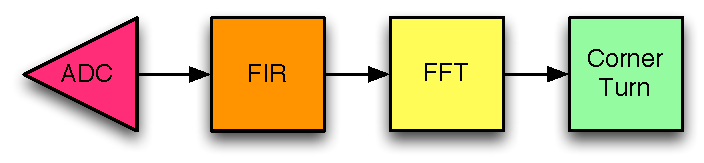
\includegraphics[width=0.48\textwidth]{Images/C4/fx_f_engine.pdf}
  \caption{FX Correlator F-Engine Model}
  \label{fig: C4/fx_f_engine.pdf}
\end{figure}

An F-Engine, pictured in Figure \ref{fig: C4/fx_f_engine.pdf} is responsible for channelizing the data from a single antenna. 
%TODO: explain or reference PFB (should be explained in C2 or 3?)
It takes in data from an ADC, and channelizes the data using a FIR and FFT to create a polyphase filter bank. 
The number of F-Engines in the correlator dataflow will vary with the number of antennas.

%TODO: add detection step
\begin{figure}[h!]
  \centering
    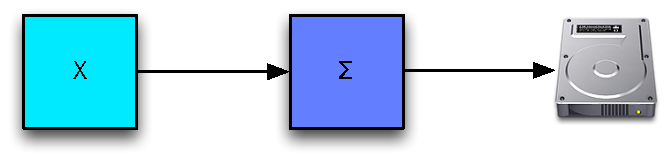
\includegraphics[width=0.48\textwidth]{Images/C4/fx_x_engine.pdf}
  \caption{FX Correlator X-Engine Model}
  \label{fig: C4/fx_x_engine.pdf}
\end{figure}

The second pipeline, the X-Engine processes the channelized data. 
Each X-Engine takes a single channel of data from every antenna in the array, cross-correlates the data, accumulates it and stores it to disk. 
Figure \ref{fig: C4/fx_x_engine.pdf} shows the pipeline for a single X-Engine. 
Since each X-Engine only operates on a single channel, the total number of X-Engines in the correlator must be the same as the number of channels in the FFT.

%TODO: add detection step
\begin{figure}[h!]
  \centering
    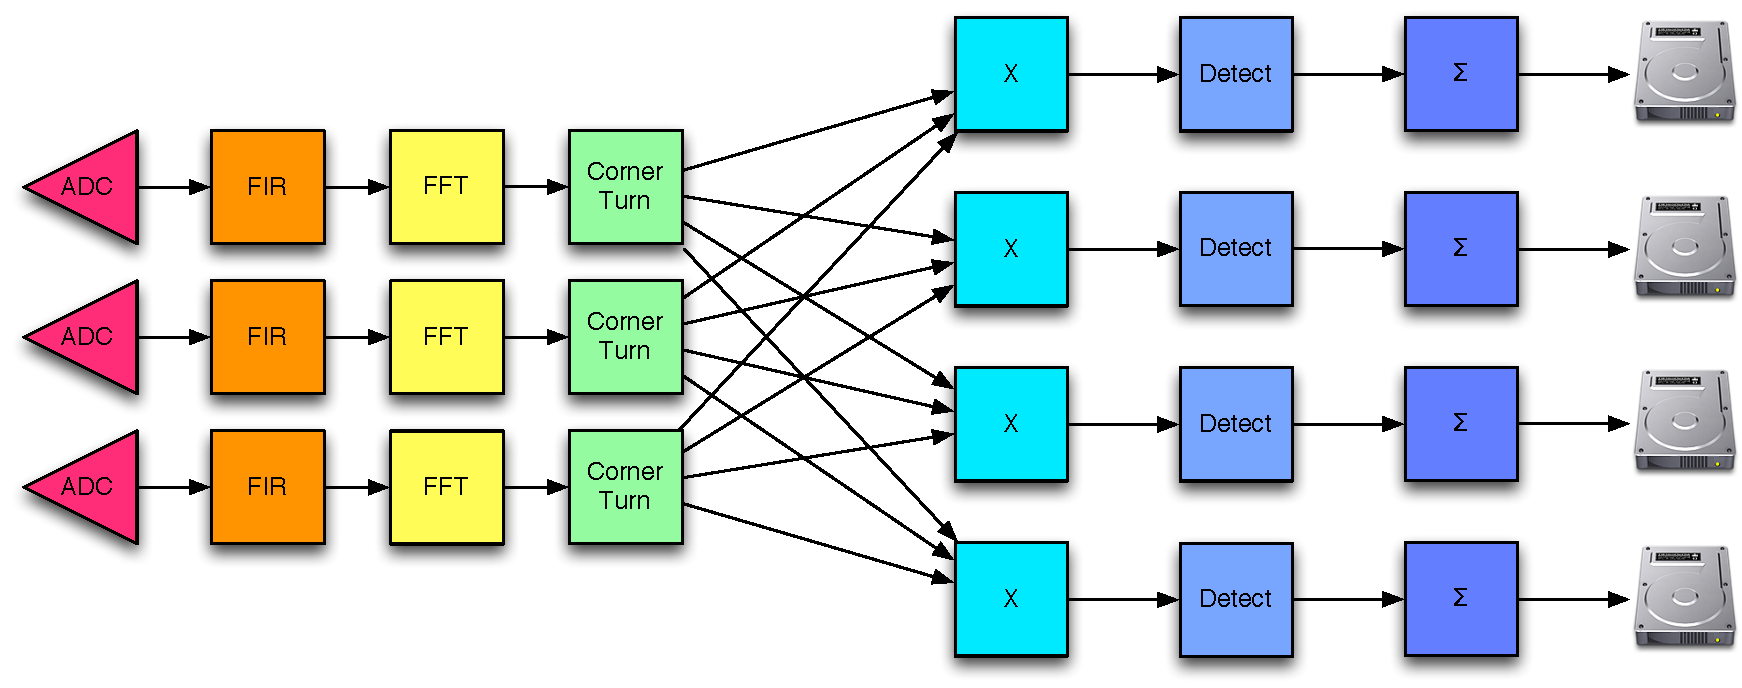
\includegraphics[width=1\textwidth]{Images/C4/fx_dataflow.pdf}
  \caption{Example FX Correlator Dataflow Model}
  \label{fig: C4/fx_dataflow.pdf}
\end{figure}

The dataflow for an FX correlator will vary quite a bit based on the input parameters. 
Figure \ref{fig: C4/fx_dataflow.pdf} shows an example there antenna four channel FX correlator. 
The left half of the figure has three F-engines, for each of the three antennas.
The right half has four X-engines, one for each channel.
And in the center, since each X-engine requires data from every F-engine, the cross-correlation blocks, represented by an \emph{X} and the FFT blocks are connected in an all-to-all configuration.



%xgpu benchmarks, correlator placement
%
%Need benchmarks for xengine
%
%HERA Correlator
%
%572 ant dual pol (currently can run in under 5 minutes)
%
%100 MHz
%
%1024 channels
%
%FPGA F, xGPU X
%
%LWA @ OVRO
%
%10k ant dual pol
%
%120k signals
%
%60MHz
%
%4096 channels
%
%1MWatt est w/GPU x-engine
%
%SKA
%
%4000 ant (8k signals)
%
%10 GHz
%
%16k channels




%\subsection{Cost}
%\subsection{Power}
%
%\section{Model Scaling}
%What about really big stuff?
%
%\section{Mixed Cost Models}
%Discuss mixing power+price
